\documentclass[a4paper, 11pt, oneside]{article}

\usepackage[utf8]{inputenc}
\usepackage[T1]{fontenc}
\usepackage[english]{babel}
\usepackage{array}
\usepackage{shortvrb}
\usepackage{listings}
\usepackage[fleqn]{amsmath}
\usepackage{amsfonts}
\usepackage{fullpage}
\usepackage{enumerate}
\usepackage{enumitem}
\usepackage{graphicx}
\usepackage{subfigure}
\usepackage{alltt}
\usepackage{indentfirst}
\usepackage{eurosym}
\usepackage{listings}
\usepackage{titlesec, blindtext, color}
\usepackage{float}
\usepackage[colorlinks, linkcolor=blue]{hyperref}
\usepackage[nameinlink,noabbrev]{cleveref}

\usepackage{titling}
\renewcommand\maketitlehooka{\null\mbox{}\vfill}
\renewcommand\maketitlehookd{\vfill\null}

\definecolor{mygray}{rgb}{0.5,0.5,0.5}
\definecolor{pink1}{rgb}{0.858, 0.188, 0.478}
\definecolor{sienna}{rgb}{0.53, 0.18, 0.09}
\definecolor{sepia}{rgb}{0.44, 0.26, 0.08}
\definecolor{midnightblue}{rgb}{0.1, 0.1, 0.44}

\renewcommand{\lstlistingname}{Code}

\lstset{
    language=C, % Utilisation du langage C
    commentstyle={\color{MidnightBlue}}, % Couleur des commentaires
    frame=single, % Entoure le code d'un joli cadre
    rulecolor=\color{black}, % Couleur de la ligne qui forme le cadre
    numbers=left, % Ajoute une numérotation des lignes à gauche
    numbersep=5pt, % Distance entre les numérots de lignes et le code
    numberstyle=\tiny\color{mygray}, % Couleur des numéros de lignes
    basicstyle=\tt\footnotesize, 
    tabsize=3, % Largeur des tabulations par défaut
    extendedchars=true, 
    captionpos=b, % sets the caption-position to bottom
    texcl=true, % Commentaires sur une ligne interprétés en Latex
    showstringspaces=false, % Ne montre pas les espace dans les chaines de caractères
    escapeinside={(>}{<)}, % Permet de mettre du latex entre des <( et )>.
    inputencoding=utf8,
    literate=
  {á}{{\'a}}1 {é}{{\'e}}1 {í}{{\'i}}1 {ó}{{\'o}}1 {ú}{{\'u}}1
  {Á}{{\'A}}1 {É}{{\'E}}1 {Í}{{\'I}}1 {Ó}{{\'O}}1 {Ú}{{\'U}}1
  {à}{{\`a}}1 {è}{{\`e}}1 {ì}{{\`i}}1 {ò}{{\`o}}1 {ù}{{\`u}}1
  {À}{{\`A}}1 {È}{{\`E}}1 {Ì}{{\`I}}1 {Ò}{{\`O}}1 {Ù}{{\`U}}1
  {ä}{{\"a}}1 {ë}{{\"e}}1 {ï}{{\"i}}1 {ö}{{\"o}}1 {ü}{{\"u}}1
  {Ä}{{\"A}}1 {Ë}{{\"E}}1 {Ï}{{\"I}}1 {Ö}{{\"O}}1 {Ü}{{\"U}}1
  {â}{{\^a}}1 {ê}{{\^e}}1 {î}{{\^i}}1 {ô}{{\^o}}1 {û}{{\^u}}1
  {Â}{{\^A}}1 {Ê}{{\^E}}1 {Î}{{\^I}}1 {Ô}{{\^O}}1 {Û}{{\^U}}1
  {œ}{{\oe}}1 {Œ}{{\OE}}1 {æ}{{\ae}}1 {Æ}{{\AE}}1 {ß}{{\ss}}1
  {ű}{{\H{u}}}1 {Ű}{{\H{U}}}1 {ő}{{\H{o}}}1 {Ő}{{\H{O}}}1
  {ç}{{\c c}}1 {Ç}{{\c C}}1 {ø}{{\o}}1 {å}{{\r a}}1 {Å}{{\r A}}1
  {€}{{\euro}}1 {£}{{\pounds}}1 {«}{{\guillemotleft}}1
  {»}{{\guillemotright}}1 {ñ}{{\~n}}1 {Ñ}{{\~N}}1 {¿}{{?`}}1
}


\newcommand{\ClassName}{INFO-0940: Operating Systems}
\newcommand{\ProjectName}{Project 2: Adding system calls - Report}
\newcommand{\AcademicYear}{2020 - 2021}

%%%% Page de garde %%%%

\title{\ClassName\\\vspace*{0.8cm}\ProjectName\vspace{0.8cm}}
\author{Goffart Maxime \\180521 \and Joris Olivier \\ 182113}
\date{\vspace{1cm}Academic year \AcademicYear}

\begin{document}

%%% Page de garde %%%
\begin{titlingpage}
{\let\newpage\relax\maketitle}
\end{titlingpage}

%%%%%%%%%%%%%%%%%%%%%%%%%%%%%%%%%%%%%%%%%%%%%%

\section{Implementation}
\paragraph{}First, we had to make the kernel aware of the 2 new system calls. Thus, we had to modify to existing files: \texttt{arch/x86/entry/syscalls/syscall\_32.tlb} and \texttt{include/linux/syscall.h}.

\paragraph{}Afterwards, we had to implement the 2 new system calls. In order to be able to retrieve the files easily, we decided to put all our new files inside a folder \texttt{custom/} at the root of the source code. This folder contains 1 file per system call and 2 files (module \& header) that allow to fetch processes that have a given name and store the pages that are read-only and present in memory.

\paragraph{}When calling \texttt{getnbpages}, we are calling the \texttt{find\_proccesses} function\footnote{Implemented in custom/get\_processes.c.} that will fetch the processes that have a name matching the given one and will store the pages that are read-only and present in memory of these processes. The return of this function is a structure \texttt{task\_struct\_list}\footnote{Defined in custom/get\_processes.h.}.\\
As explained in \autoref{section2}, we need to check all the \texttt{task\_struct} inside the kernel memory, in order to find the processes that have a name matching the given one, because each one represents a process. When we have the list of the processes that we are considering, we need to go through all their \texttt{vm\_area\_struct} because each one of these represents multiple pages. For each page, we need to check if it is read-only and present in memory. If it is the case, we are storing it in order to be able to set the bitmap in the \texttt{getreadpages} system call.\\
The structure \texttt{task\_struct\_list} is a linked list of \texttt{task\_struct\_list\_node} where each one of the latter represents a process that have a name equal to the given one. Each \texttt{task\_struct\_list\_\\node} contains a linked list of \texttt{page\_list} which represents a read-only page that is present in memory.\\
In order to be able to access the generated structure when calling \texttt{getreadpages}, we are storing a pointer to it inside the \texttt{mm\_struct} of the process with pid equal to 1 (systemd).

\paragraph{}When calling \texttt{getreadpages}, we are fetching the pointer stored inside the \texttt{mm\_struct} of process with pid 1 and checking if the process's name on which getnbpages was called is the same as the one provided. Then, we have to walk across the linked lists that were stored. The top-level linked list store one linked list per process with the embedded linked list storing the pages that read-only and present in memory. Each node inside the embedded linked list store the index of the page. Thus, by walking through all the linked lists, we are able to fetch all the indexes that should be set to 1 inside the bitmap.

\section{How the memory of a process is managed by the kernel ?}\label{section2}

\paragraph{}Processes are implemented in the kernel as instances of \texttt{task\_struct}. 
This struct contains a \textit{mm} field which is an instance of \texttt{mm\_struct} that represents a 
summary of the process memory. This \textit{mm} field contains a \textit{mmap} field that is an instance of \texttt{vm\_area\_struct} that represents 
a memory area. This \textit{mmap} field contains 3 fields \textit{vm\_start}, \textit{vm\_end}, and \textit{vm\_next}. The first one represents the logical 
address corresponding to the first address within the virtual memory area, the second one represents the first address outside the virtual memory area, and the 
third one is a reference to another \texttt{vm\_area\_struct} which contains higher segment begin and end addresses. 

\paragraph{}To translate a logical address to a physical address, a page table is used. This table allows 
to obtain the physical address corresponding to a given logical address using multi-level paging in order to reduce the size of the table that is stored in physical memory.
Moreover, the offset of the logical address is retained according to the page size and only the first bits of the logical address are used to look at the mapping in the table in order to 
reduce the size of the entries in the table. Some entries do not refer to any physical page: this means that they have the present flag clear. This could be because their contents have been swapped out or because they never have been touched.

\paragraph{}This management of the process memory by the kernel is represented on the \autoref{fig:kernel_memo}.
\begin{figure}[H]
  \centering
  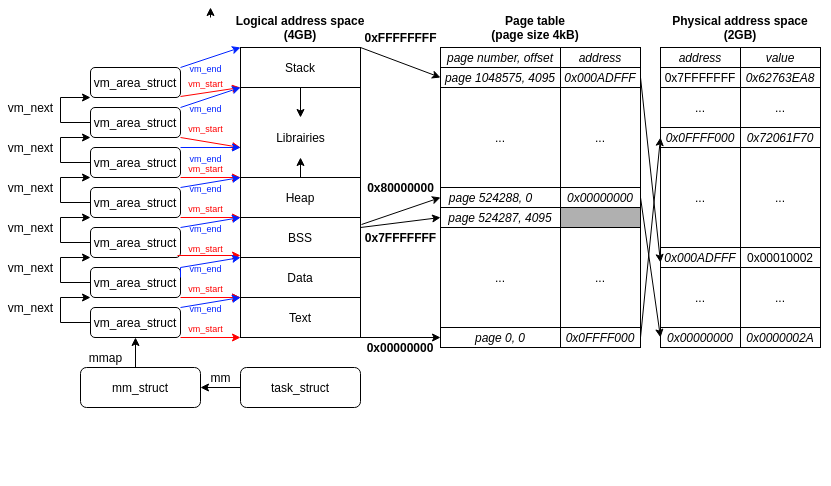
\includegraphics[scale=0.6]{kernel_memo.png}
  \caption{Management of the process memory by the kernel.}\label{fig:kernel_memo}
\end{figure}

\section{Time spent}
\paragraph{}Considering the time spent on research before starting the implementation, the implementation, testing, and making the report, Olivier spent approximately \texttt{x} hours and Maxime spent approximately 17 hours.

\end{document}
